\chapter{Programando o Terminal Gráfico/IHM}
\label{chap:resultados}


A programação do terminal gráfico pode ser tão comlexa quanto mais recursos forem utilizados, 
passando por sistemas de identificação de usuários, 
conexão com banco de dados, 
validação de informações, 
multiplas conexões, 
segurança, 
entre outras possibilidades que o software de programação permite. 
A abordagem aqui tem o intuito de promover os primeiro passos com o uso da ferramenta, 
a criação das primeiras telas, 
a navegação e a acomunicação com um controlador. 
Sendo assim, são abordadas apenas as etapas de criação do projeto,
configuração do controlador através das TAGs e 
do protocolo de comunicação, 
a elaboração de telas de navegação e visualização de informações e
o envio do projeto para o terminal gráfico que estamos trabalhando.


\section{Criando um projeto}

A criação de um projeto para o terminal gráfico da série iX, 
entre outras, 
é o iX Developer que pode ser baixado gratuitamente em 
\cite{terminais_operacao_serie_ix}, 
com a possibilidade de uso completo pelo período de teste de 30 dias.

A versão utilizada para a produção deste documento foi a 2.20, 
que pode ser vista na Figura \ref{fig:new_project}, 
que é a tela inicial ao abrir o software. 


\begin{figure}[ht!]
	\centering
	\Caption{\label{fig:new_project}Criando um novo projeto com iX Developer }
	\UECEfig{}{\fbox{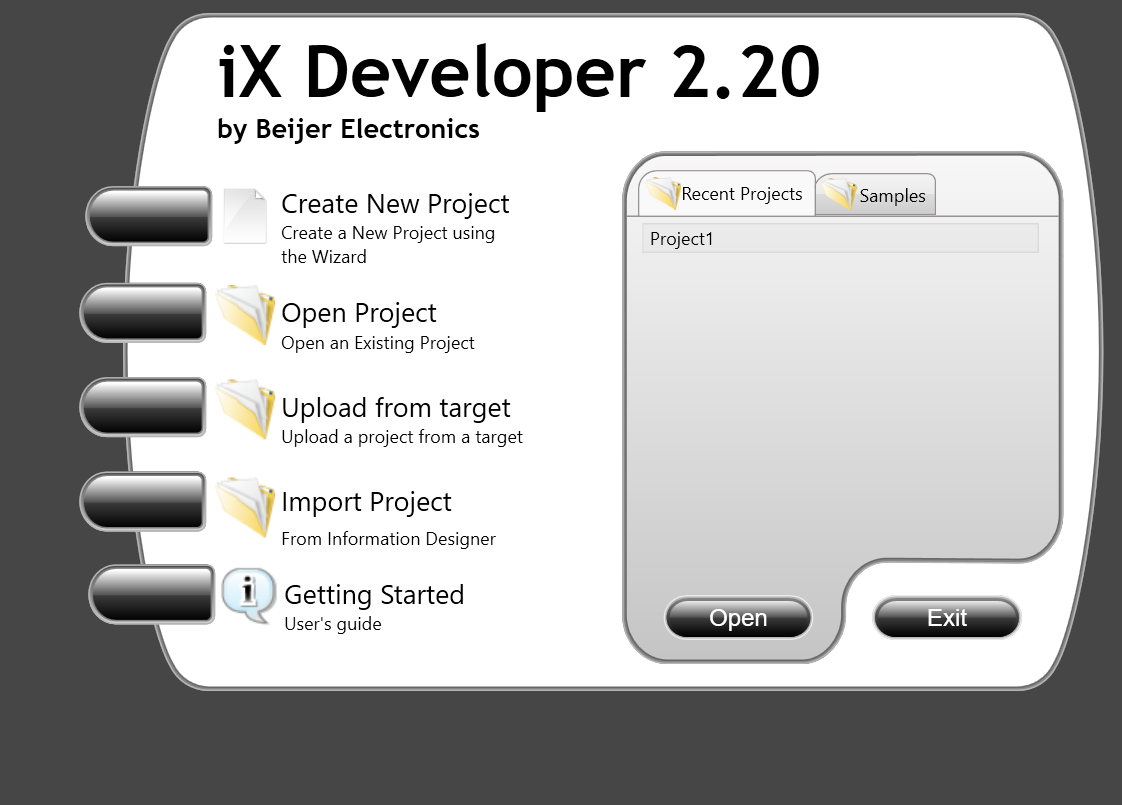
\includegraphics[width=8cm]
		{figuras/ix-new_project} 
		}}{ \Fonte{Elaborado pelo autor}    }
\end{figure}

Nesta tela inicial, algumas tarefas são possíveis, 
como abrir um projeto existente, 
ou mesmo consultar um guia de usuário. 
Para a criação de um novo projeto clique em 
\textit{\textbf{Create New Project}}.


A Figura \ref{fig:choose_target} 
ilustra a tela seguinte em que é necessário indicar o modelo de IHM que estamos utilizando. 


\begin{figure}[ht!]
	\centering
	\Caption{\label{fig:choose_target}Escolhendo um terminal gráfico }
	\UECEfig{}{\fbox{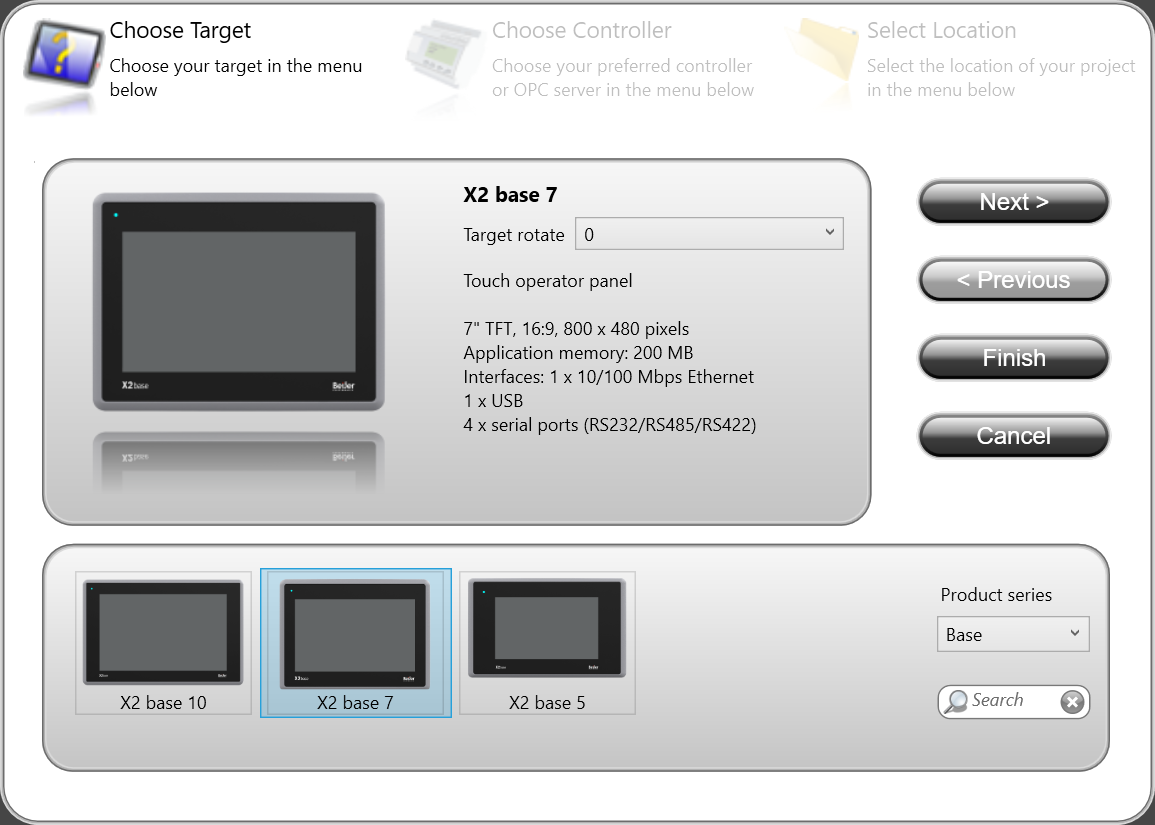
\includegraphics[width=8cm]
		{figuras/ix-choose_target } 
		}}{ \Fonte{Elaborado pelo autor}    }
\end{figure}


O modelo de terminal gráfico iX-T7F-2 foi descontinuado, 
e não há suporte no software, 
mas de acordo com a Notificação de Regime de Produção 
\cite{ix_t7f_2-x2_base_7} 
pode-se utilizar o modelo equivalente que é o 
\textbf{X2-BASE-7}, conforme selecionado na própria imagem.

Após a seleção do modelo, clique em \textbf{\textit{Next>}}.

A seleção seguinte é do controlador, que neste caso, 
significa escolher um protocolo de comunicação com a IHM. 

Selecione então \textbf{MODICON}, 
que é a desenvolvedora do protocolo Modbus, 
e deve ser selecionada na janela ao lado. 
Tomaremos a IHM como o \textbf{Cliente} da comunicação, 
então selecione \textbf{Modbus Master}.  



\begin{figure}[ht!]
	\centering
	\Caption{\label{fig:choose_controller}Escolhendo um protocolo de comunicação e uma marca de controlador}
	\UECEfig{}{\fbox{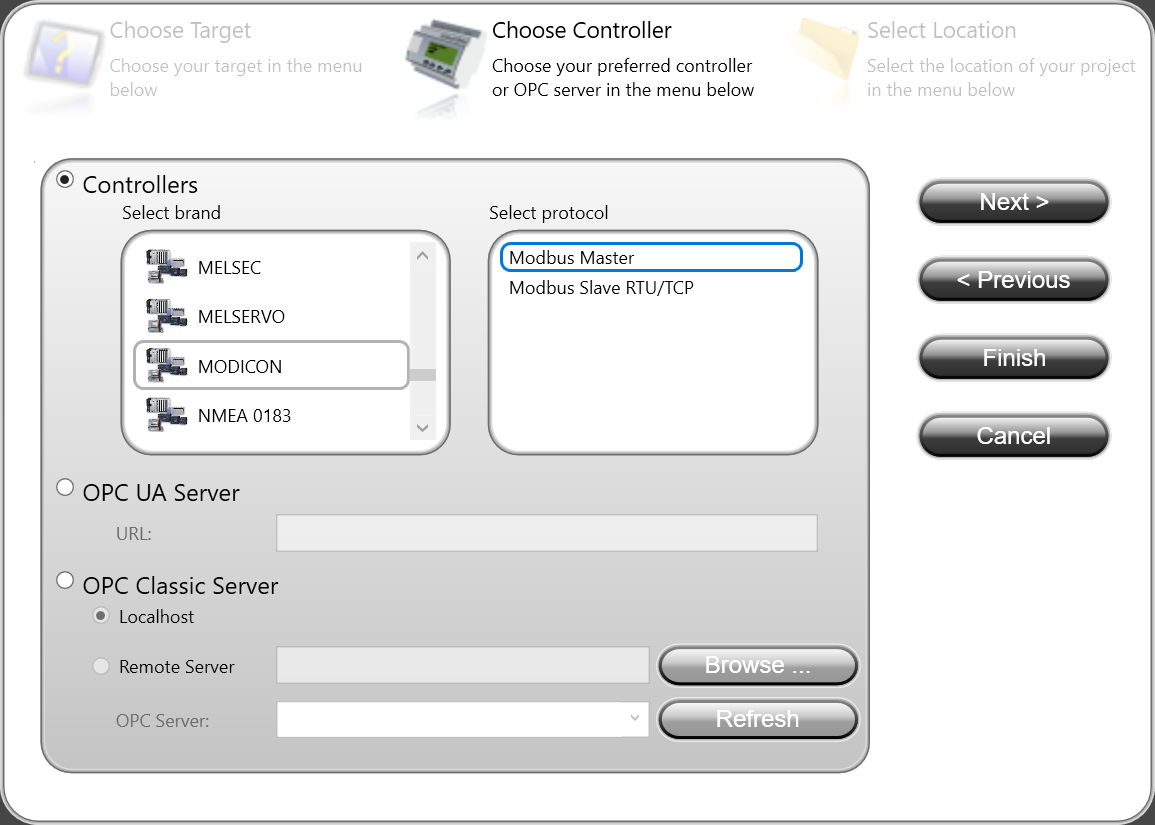
\includegraphics[width=8cm]
		{figuras/ix-choose_controller } 
		}}{ \Fonte{Elaborado pelo autor}    }
\end{figure}


Após a seleção do protocolo de comunicação, 
clique em \textbf{\textit{Next>}}.

A etapa final consiste na escolha de um local de armazenamento
e da escolha de um nome ao projeto, 
conforme Figura \ref{fig:select_location}.

\begin{figure}[ht!]
	\centering
	\Caption{\label{fig:select_location}Seleção de local de armazenamento do projeto }
	\UECEfig{}{\fbox{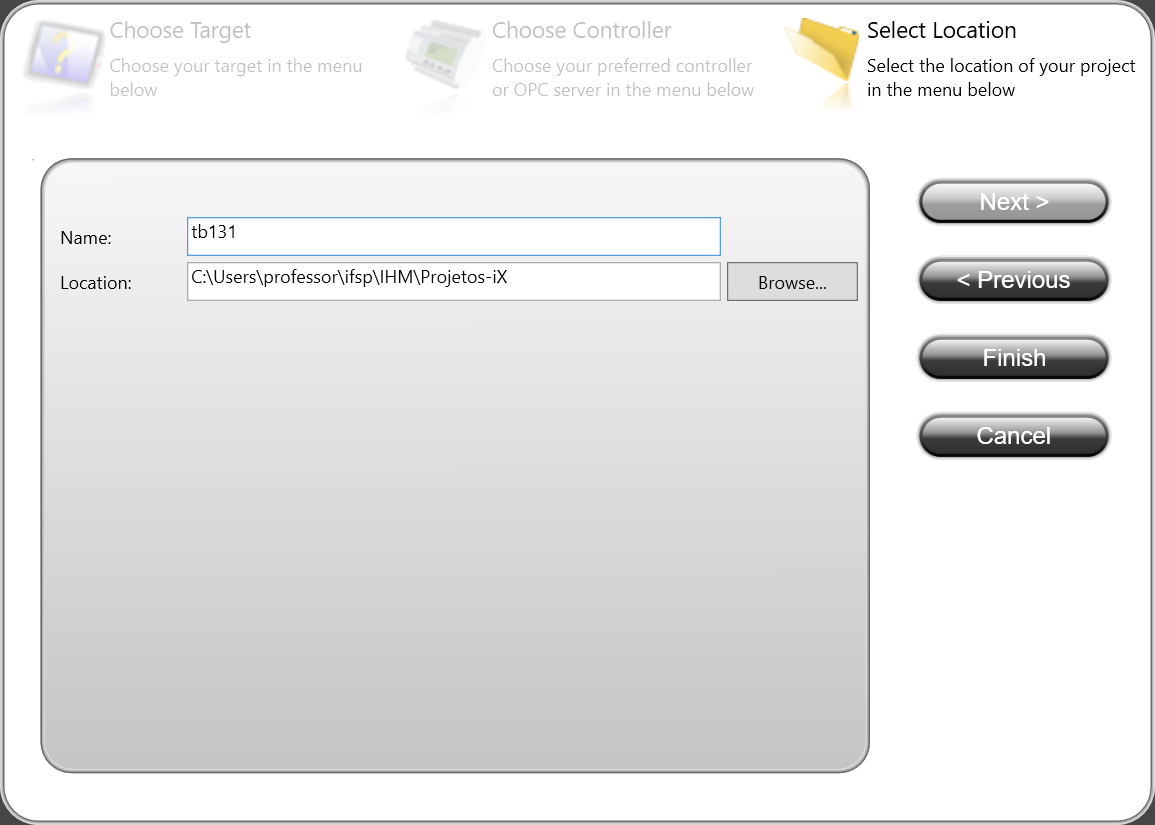
\includegraphics[width=8cm]
		{figuras/ix-select_location } 
		}}{ \Fonte{Elaborado pelo autor}    }
\end{figure}

Após a definição de local e nome do projeto 
clique em \textbf{\textit{Finish}}.

A Figura \ref{fig:screen1} 
ilustra a tela inicial para a criação de um projeto. 


\begin{figure}[ht!]
	\centering
	\Caption{\label{fig:screen1}Tela inicial ao criar um novo projeto}
	\UECEfig{}{\fbox{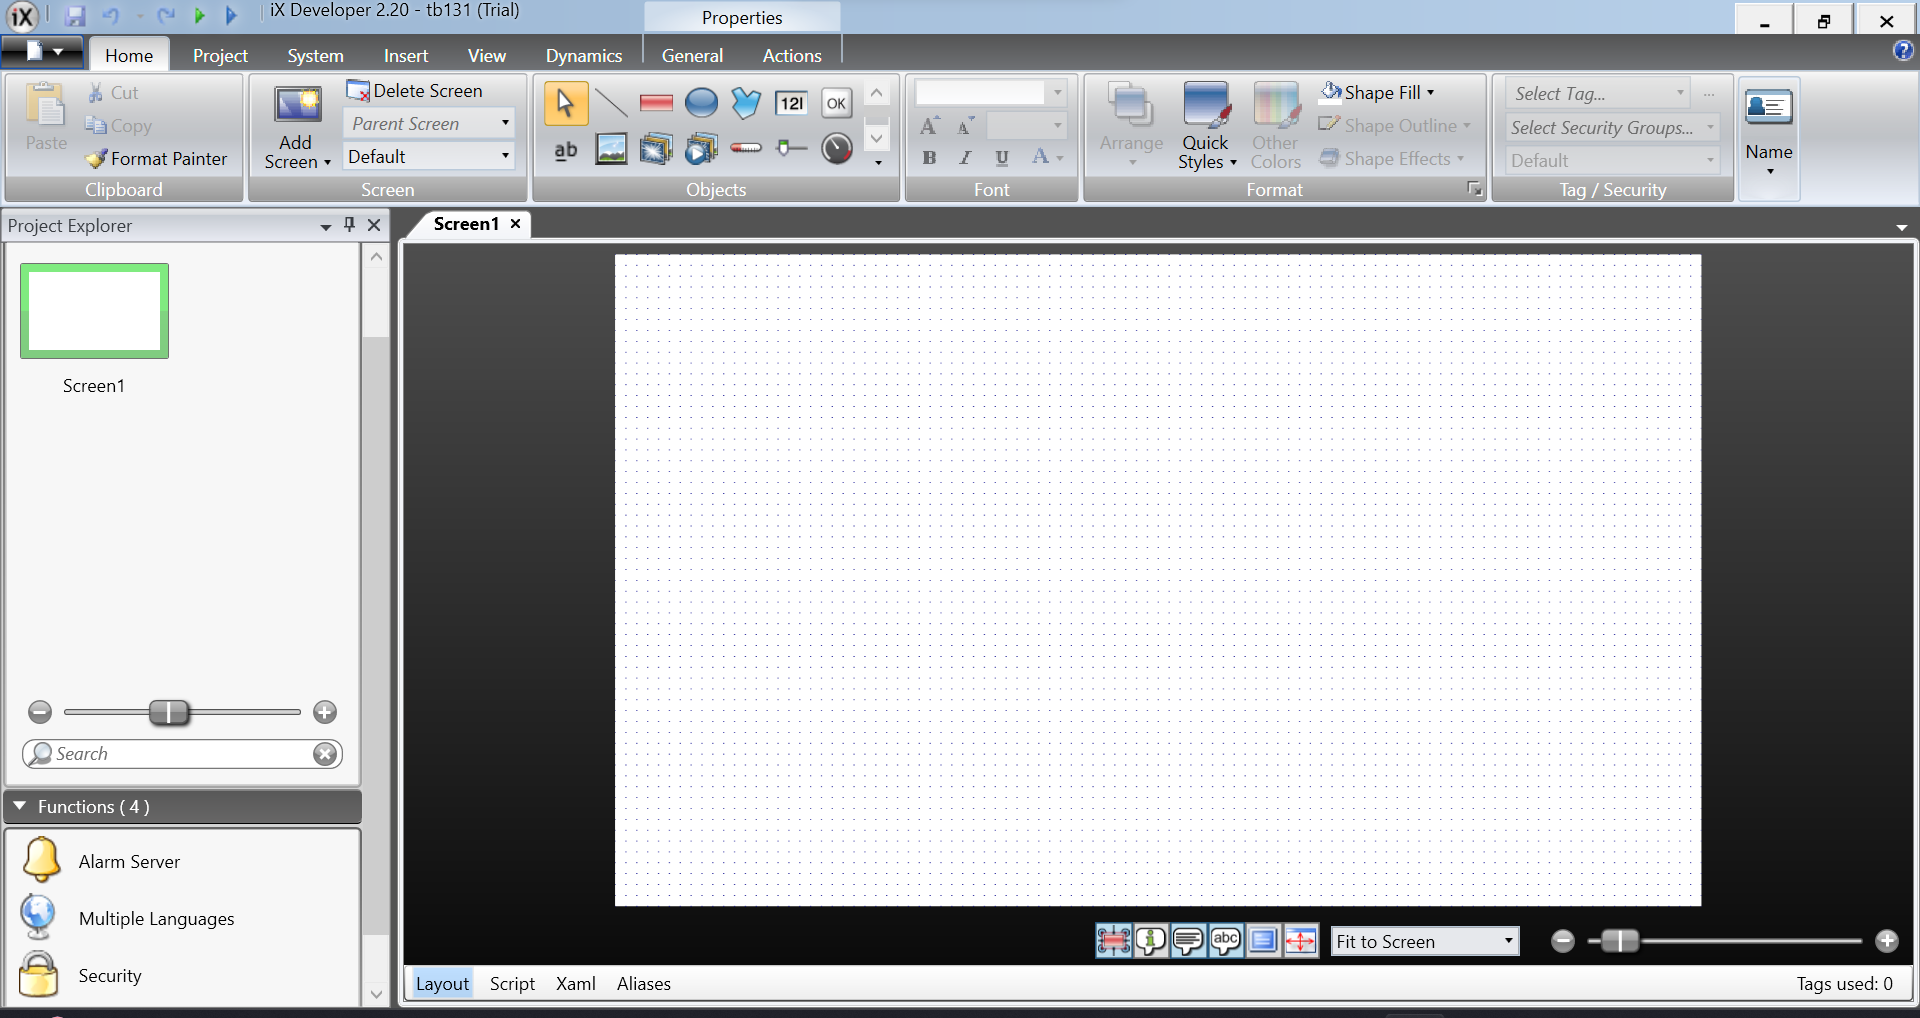
\includegraphics[width=14cm]
		{figuras/ix-screen1} 
		}}{ \Fonte{Elaborado pelo autor}    }
\end{figure}





\section{Configurando TAGs}


Após a criação do projeto, 
recomenda-se iniciar pela declaração de TAGs, 
que são as variáveis, que conectam os elementos gráficos com as respectivas variáveis do controlador. 

A Figura \ref{fig:functions-tags} 
ilustra a sequência de passos para a declaração das TAGs. 
Ao clicar na opção \textbf{Tags} 
no quadro \textbf{Functions}, 
\textbf{indicador 1}, 
na tela principal abre-se uma aba para a declaração das Tags, 
\textbf{indicador 2}.



\begin{figure}[ht!]
	\centering
	\Caption{\label{fig:functions-tags} Incluindo TAGs ao projeto }
	\UECEfig{}{\fbox{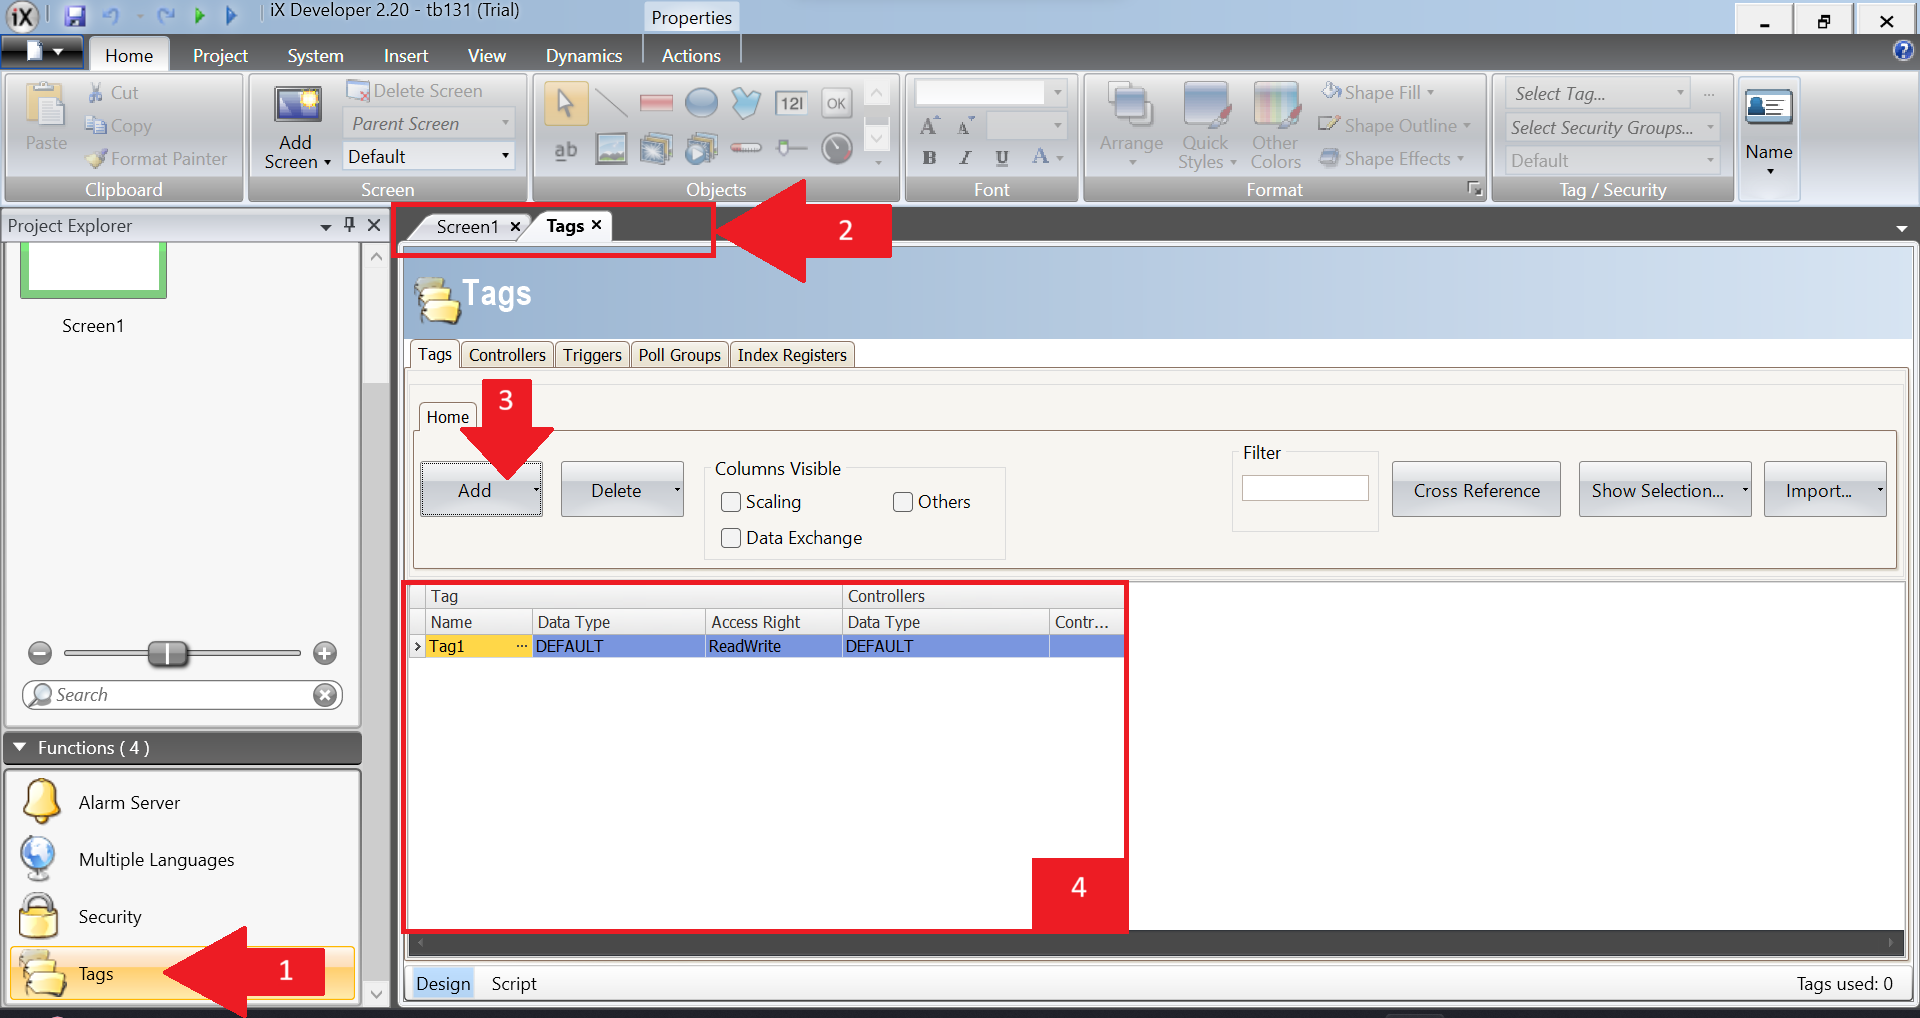
\includegraphics[width=14cm]
		{figuras/ix-functions-tags-n } 
		}}{ \Fonte{Elaborado pelo autor}    }
\end{figure}



Clicando em \textbf{Add}, \textbf{indicador 3}, 
são adicionadas TAGs no quadro do \textbf{indicador 4}. 
Todas as variáveis do controlador que forem ser representadas ou manipuladas de alguma forma, devem ser declaradas como TAGs. 


A Figura \ref{fig:tags} 
ilustra as TAGs envolvidas no projeto para a comunicação com o TB131. 
O conjunto de TAGs possui três propriedades, 
\textbf{Nome}, \textbf{Tipo de Dado} e \textbf{Direito de Acesso}.
De forma correlata, 
cada TAG possui um respectivo endereço Modbus e seu tipo. 



\begin{figure}[ht!]
	\centering
	\Caption{\label{fig:tags} As Tags do projeto }
	\UECEfig{}{\fbox{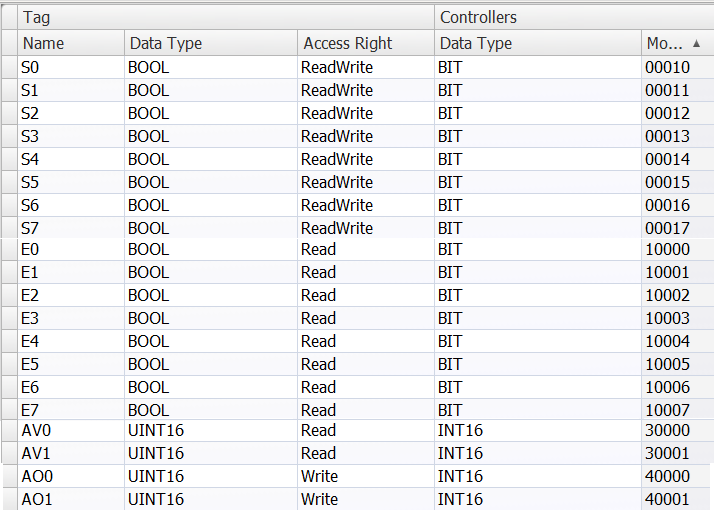
\includegraphics[width=10cm]
		{figuras/ix-tags-n } 
		}}{ \Fonte{Elaborado pelo autor}    }
\end{figure}


As variáveis de saída do TB131 
são ligados às variáveis nomeadas de S0 a S7, 
do tipo Booleana e com direito de acesso a leitura e escrita. 
Os endereços Modbus são associados às funções, 
representados em hexadecimal com os valores de 00010h até 00017h,
para acesso às \textit{Coils}, ou seja, as saídas digitais ou bobinas no CLP. 

As variáveis de entrada do TB131 
são ligadas às variáveis nomeadas de E0 até E7, 
do tipo Booleana e com direito de acesso somente a leitura. 
Os endereço Modbus estão no intervalo 10000h até 10007h, 
para Discrete Inputs, ou seja, as entradas digitais.

As variáveis AV0 e AV1 
são conectadas aos valores analógicos dos potenciômetros do TB131,
do tipo UINT16, inteiro de 16bits sem sinal, somente leitura. 
São endereçadas entre 30000h e 30001h. 

As variáveis AO0 e AO1 
são conectadas aos valores analógicos de saída do TB131, 
do tipo UINT16, interiro de 16bits sem sinal, somente escrita. 
São endereçadas em 40000h e 40001h. 



\begin{figure}[ht!]
	\centering
	\Caption{\label{fig:controller_settings} Parâmetros do controlador }
	\UECEfig{}{\fbox{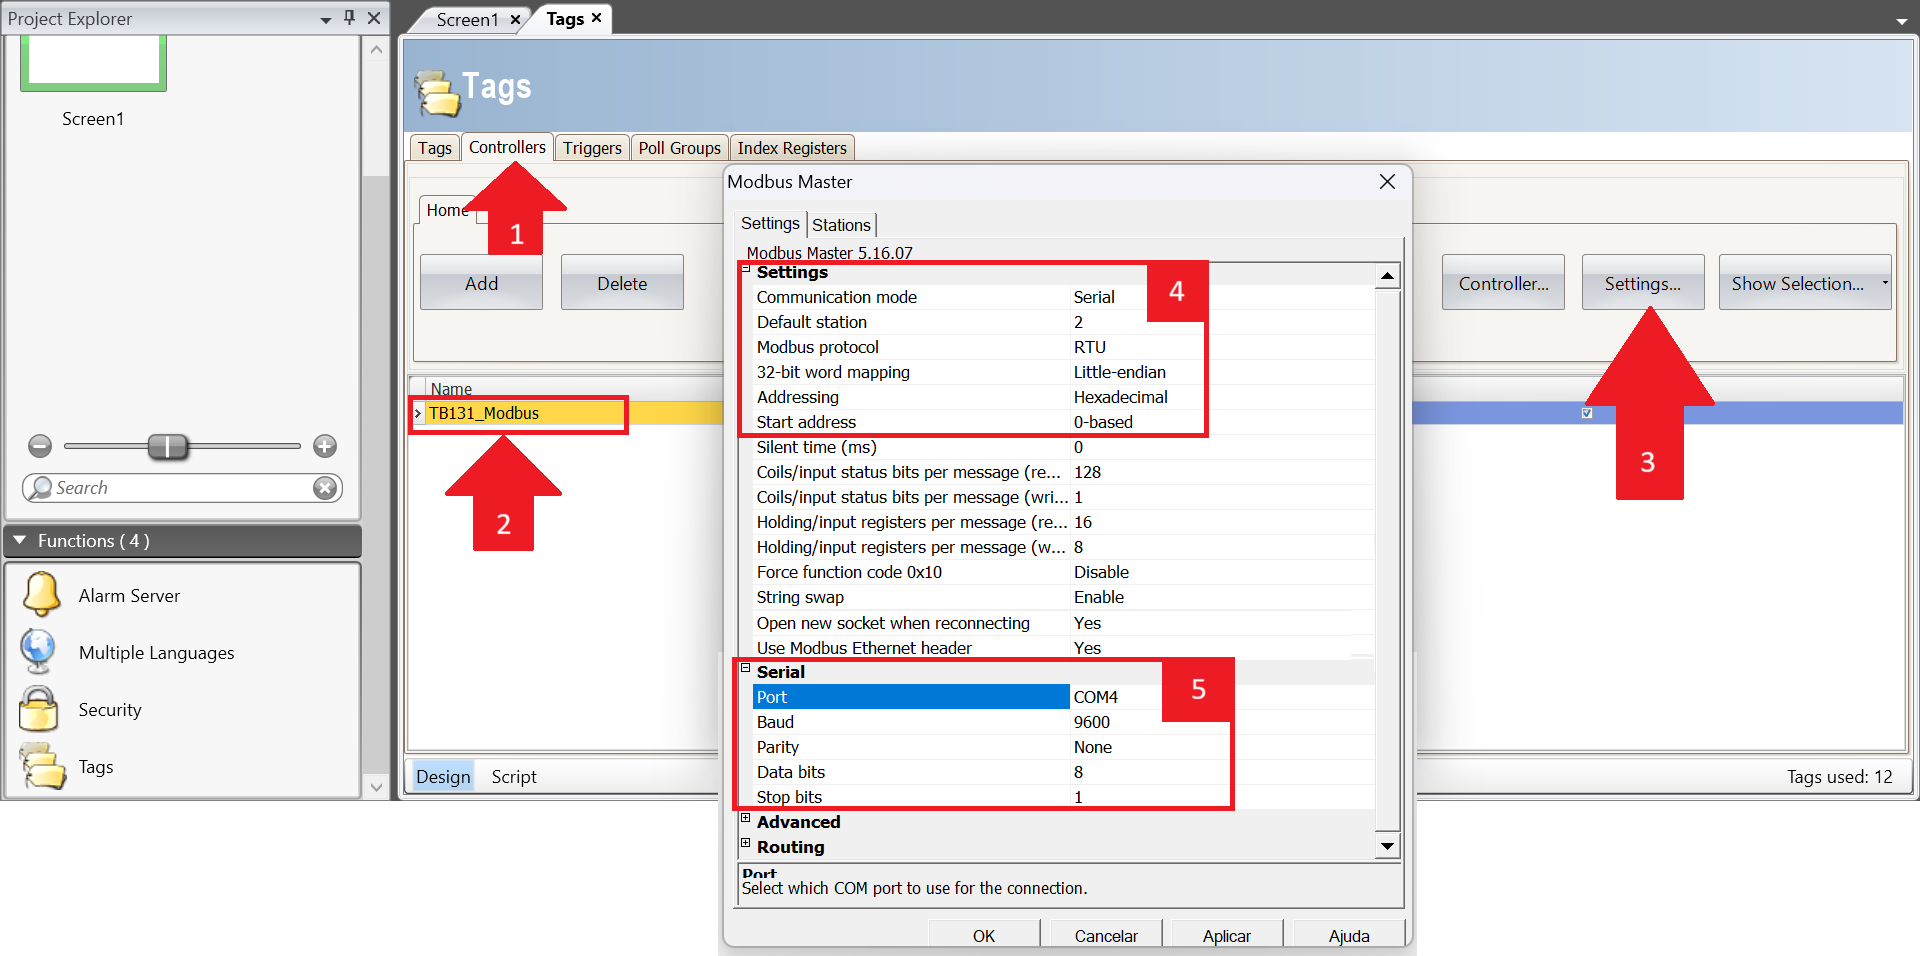
\includegraphics[width=14cm]
		{figuras/ix-controller_settings-n } 
		}}{ \Fonte{Elaborado pelo autor}    }
\end{figure}




A Figura \ref{fig:controller_settings} ilustra 
os passos da configuração da comunicação com o controlador, 
clicando no \textbf{indicador 1}.
No \textbf{indicador 2}, 
pode-se renomear o controlador, 
principalmente se houverem outros controladores envolvidos do processo. 



Clicando no \textbf{indicador 3}, 
podem ser configurados os parâmetros da comunicação Modbus, 
no \textbf{indicador 4} e da porta serial no \textbf{indicador 5}.


Além desta configuração e escolha de porta (COM2 ou COM4), 
é necessário habilitar a porta de comunicação serial que será utilizada conforme Figura \ref{fig:serial_port}. 


\begin{figure}[ht!]
	\centering
	\Caption{\label{fig:serial_port} Configurando porta de comunicação para RS485 }
	\UECEfig{}{\fbox{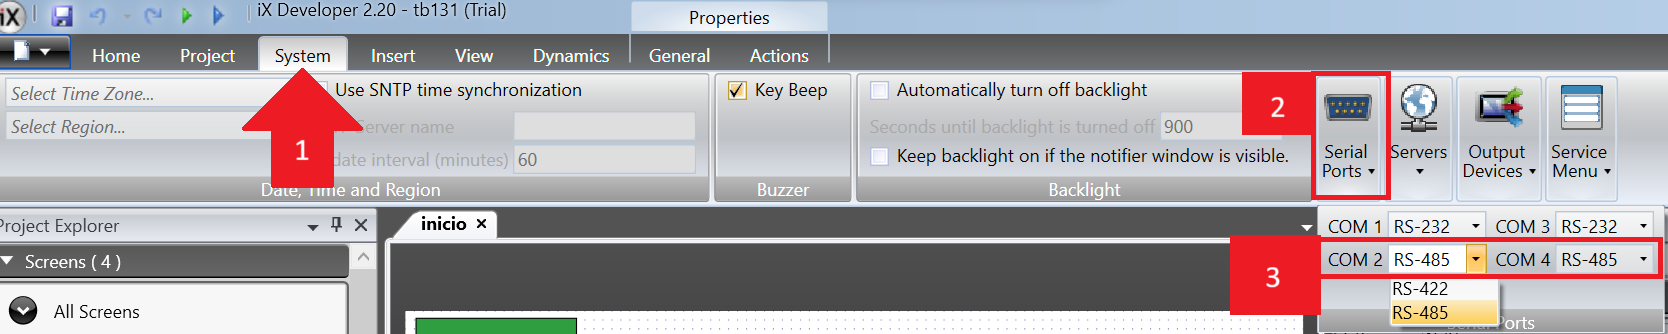
\includegraphics[width=12cm]
		{figuras/ix-serial_port-n } 
		}}{ \Fonte{Elaborado pelo autor}    }
\end{figure}

%As portas de comunicação COM1 e COM2 
%compartilham um mesmo conector, assim como COM3 e COM4. 

As portas COM2 e COM4 podem ser configuradas como RS-485 e RS-422.
No caso deste projeto, selecione a RS-485 de acordo com a porta COM selecionada anteriormente. 





\section{Inclusão de objetos gráficos}


A montagem das telas, 
basicamente acontece inserindo os elementos denominados objetos, 
que podem ser desde formas simples até indicadores com animação. 


A Figura \ref{fig:obj_properties} 
ilustra a inserção de objetos formando a primeira tela do projeto,
composta pelo logo do IFSP e de uma barra lateral na cor verde.



\begin{figure}[ht!]
	\centering
	\Caption{\label{fig:obj_properties} Propriedade dos objetos  }
	\UECEfig{}{\fbox{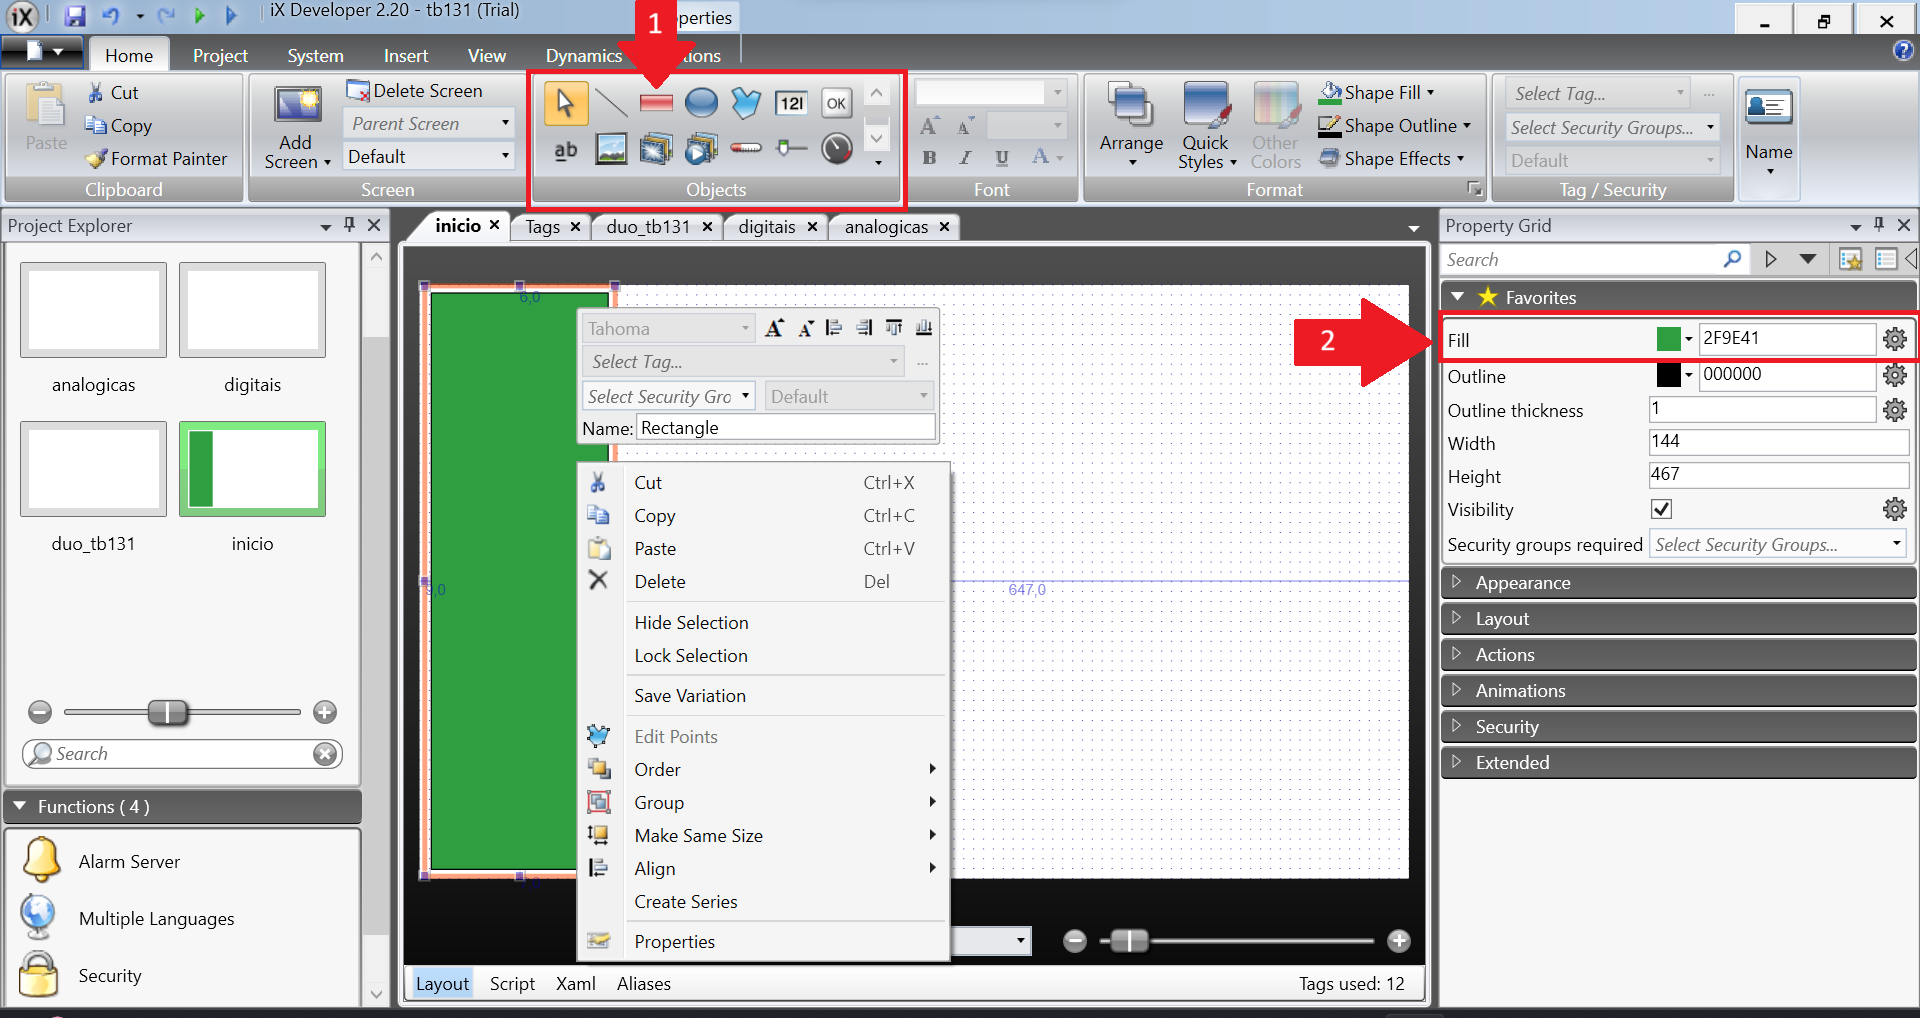
\includegraphics[width=12cm]
		{figuras/ix-objects_properties-n}
		}}{ \Fonte{Elaborado pelo autor}    }
\end{figure}


O \textbf{indicador 1} aponta o objeto utilizado, 
que é a forma retungular.
Ao cliacar com \textbf{botão direito do mouse} sobre a forma inserida, 
a opção \textit{\textbf{Properties}}, 
abre uma janela lateral com as propriedades do objeto. 

O \textbf{indicador 2} 
aponta a propriedade de cor do preenchimento, 
que está ajustada no formato RGB hexadecimal com o valor \textbf{2F9E41h}, 
que é a cor verde oficial do logo do IFSP.

Outros parâmetros podem ser ajustados a depender do visual que se queira obter. Explore!


A Figura \ref{fig:tela_inicio} 
ilustra os passos para a inserção de uma imagem externa como elemento visual da tela. 
Ao clicar no ícone, deve-se marcar um quadro na tela, 
na posição em que a imagem será inserida.
Ao fazer isso, 
abre-se uma janela de busca, 
padrão do sistema operacional, 
da mesma forma que ocorre ao salvar um arquivo. 
Após a seleção do elemento, 
ele é inserido no quadro marcado inicialmente. 
Após a inserção é possivel redimensionar o tamanho da imagem, dentre outas propriedades possíveis de edição.

\begin{figure}[ht!]
	\centering
	\Caption{\label{fig:tela_inicio} Adicionando imagem externa em uma tela }
	\UECEfig{}{\fbox{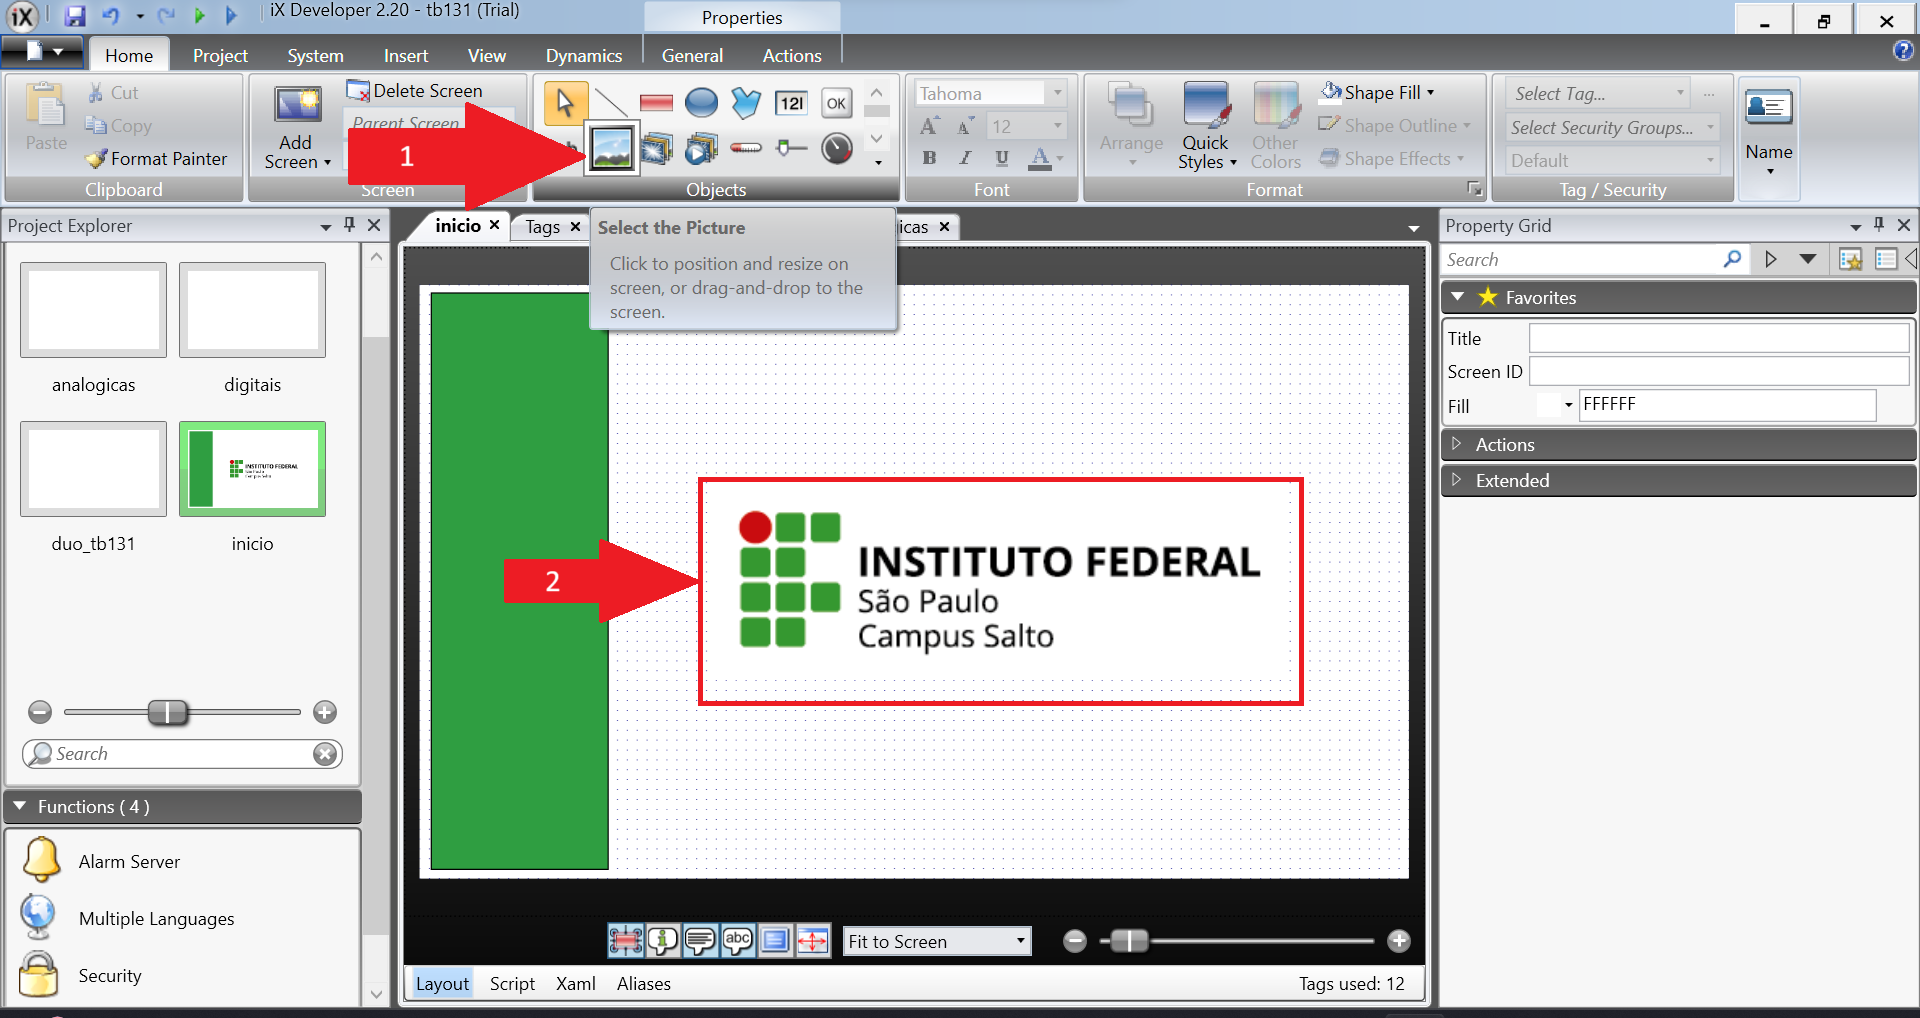
\includegraphics[width=14cm]
		{figuras/ix-tela_inicio-n}
		}}{ \Fonte{Elaborado pelo autor}    }
\end{figure}

Para a atribuição de ação ao objeto inserido na tela, 
ilustrado na Figura \ref{fig:screen_inicio},
é possivel definir que tipo de evento irá produzir a ação, 
na janela de propriedades, seção \textbf{\textit{Actions}}.



\begin{figure}[ht!]
	\centering
	\Caption{\label{fig:screen_inicio} Configurando evendo de transição de tela }
	\UECEfig{}{\fbox{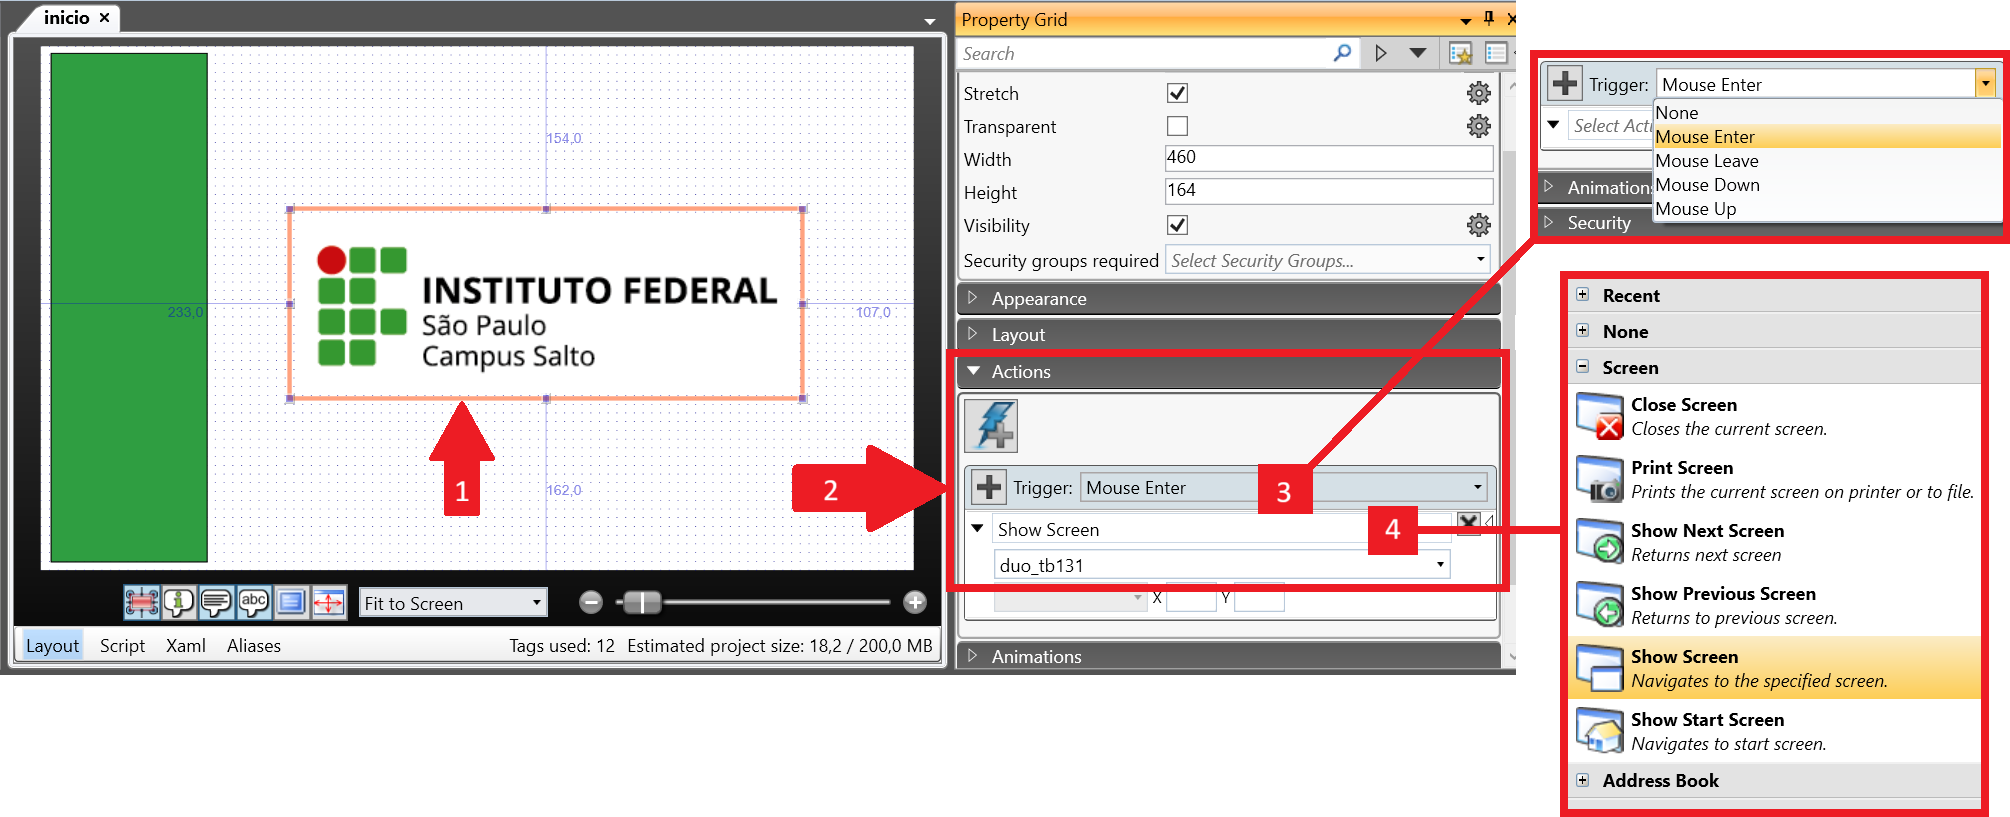
\includegraphics[width=15cm]
		{figuras/ix-screen_inicio-n}
		}}{ \Fonte{Elaborado pelo autor}    }
\end{figure}


O evendo selecionado no \textbf{indicador 3}, 
foi um \textbf{clique do mouse} no objeto, 
que dispara a ação correspondente, 
que é a transição de tela, 
conforme \textbf{indicador 4}, 
cujo último parâmetro do \textbf{indicador 2}, 
é a tela de destino. 



A Figura \ref{fig:select_polyline} 
evidencia a ferramenta denominada \textbf{Poly Line} 
que permite a produção de formas distintas às básicas, 
retangulares e circulares. 
Os trapézios retangulares utilizados como botões de transição 
às respectivas telas foram feitos utilizando esta ferramenta. 


\begin{figure}[ht!]
	\centering
	\Caption{\label{fig:select_polyline} Botões do menu principal }
	\UECEfig{}{\fbox{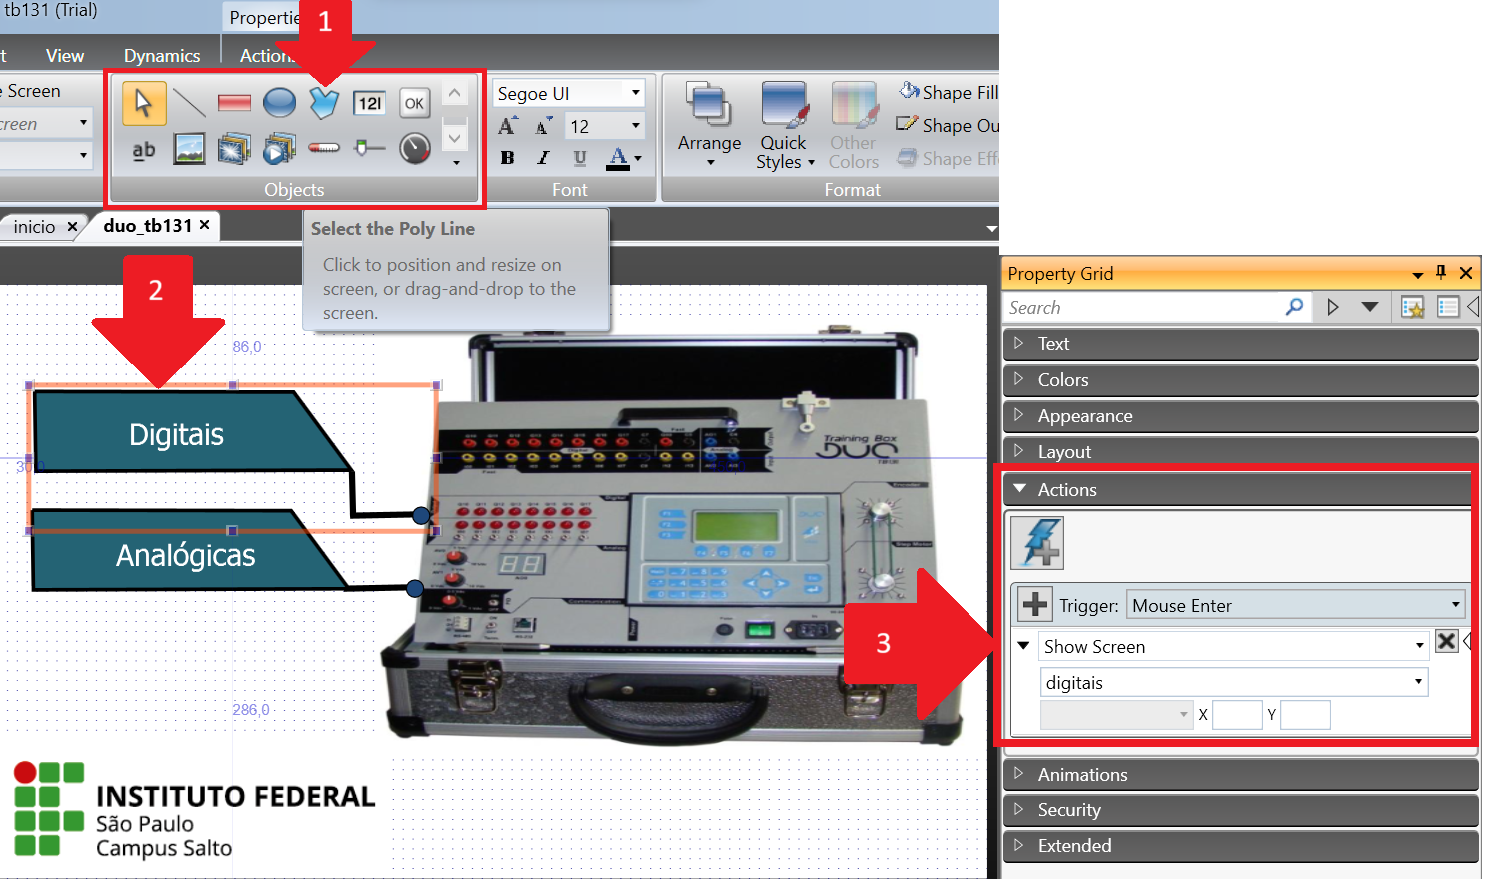
\includegraphics[width=14cm]
		{figuras/ix-screen-select_polyline-n}
		}}{ \Fonte{Elaborado pelo autor}    }
\end{figure}

A produção da transição da tela de menu para a tela das 
entradas e saídas digitais é feita de forma análoga à 
transição da tela inical. 



As entradas digitais, 
são representadas com circulos conforme 
\textbf{indicador 1} da Figura 
\ref{fig:digitais_entradas}, 
sendo um elemento com duas cores 
a depender do estado lógico da respectiva variável que este elemento representa. 

\begin{figure}[ht!]
	\centering
	\Caption{\label{fig:digitais_entradas} Configuração dos sinalizadores das entradas digitais }
	\UECEfig{}{\fbox{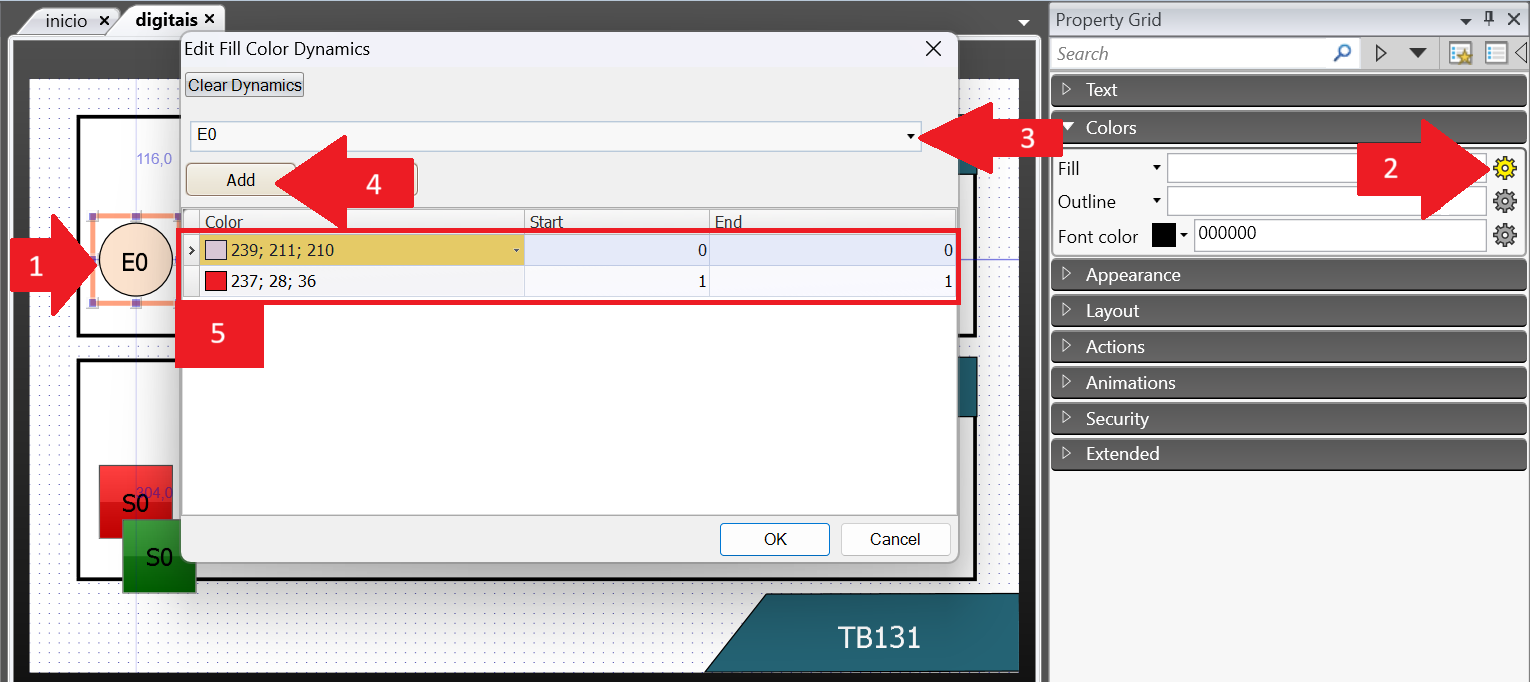
\includegraphics[width=14cm]
		{figuras/ix-digitais_entradas_fillcolor-n}
		}}{ \Fonte{Elaborado pelo autor}    }
\end{figure}

Acessando as propriedades do objeto, 
e clicando na engrenagem correspondente ao 
campo de preenchimento de cor, 
\textbf{indicador 2}, 
pode-se configurar uma variável para associar este objeto,
\textbf{indicador 3}, 
e adicionar uma cor,
\textbf{indicador 4} 
para cada estado lógico da variável,
\textbf{indicador 5}.



As saídas digitais possuem um efeito de 
ao pressionar o botão, 
mudar o estado lógico da variável e 
mudar a própria cor do botão, 
porém este efeito foi produzido utilizando 
dois botões de cor única, 
alternando a propriedade de visibilidade.


A Figura \ref{fig:digitais_saidas} 
ilustra a configuração para o botão desligar, 
na cor vermelha, 
mas o processo é o mesmo para o botão verde, 
exceto pelo estado que produz a visibilidade do objeto.


\begin{figure}[ht!]
	\centering
	\Caption{\label{fig:digitais_saidas} Configuração dos sinalizadores das saídas digitais}
	\UECEfig{}{\fbox{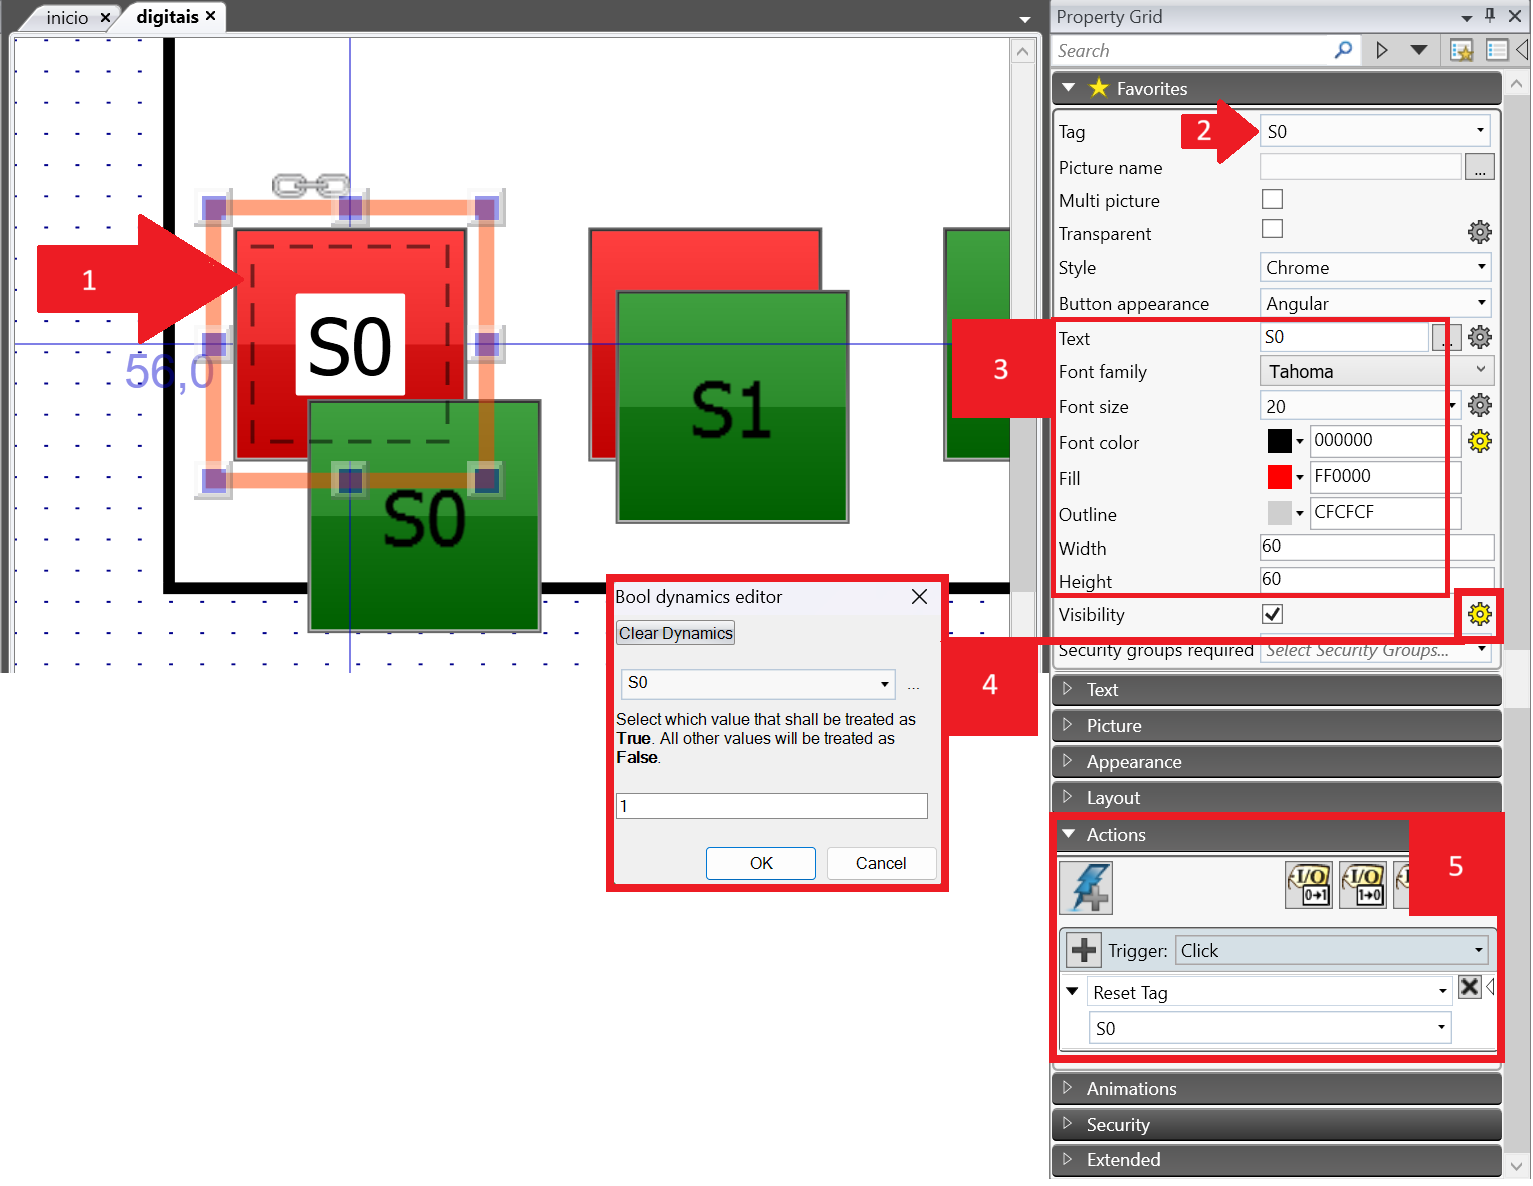
\includegraphics[width=14cm]
		{figuras/ix-digitais_saidas_vermelho-n}
		}}{ \Fonte{Elaborado pelo autor}    }
\end{figure}


O passo inicial consiste em abrir as propriedades do objeto,
\textbf{indicador 1}. 

Indicar a TAG associada ao objeto,
\textbf{indicador 2}.

Ajustar os parâmetros visuais,
\textbf{indicador 3},
como texto exibido, cor, tamanho de fonte, e dimensões do objeto.

Acessando as configurações da opção de visibilidade,
(\textbf{\textit{Visibility}}), 
deve-se novamente apontar a TAG que servirá de referência,
\textbf{indicador 4},
e qual o seu valor que condiciona a visibilidade do objeto. 
Neste caso, 
quando a variável \textbf{S0} 
possuir o valor lógico \textbf{1}, 
significa que a saída está ligada, 
e o botão vermelho irá ficar visível para uma futura ação de desligar. 

Por fim, a ação associada ao objeto,
\textbf{indicador 5},
é o \textbf{reset Tag} de \textbf{S0}, 
produzido pelo \textbf{click} no objeto.


Para o botão verde, 
os parâmetros são os mesmos, 
exceto a cor do botão e o 
estado da TAG que torna o objeto visível, 
que neste caso é o valor lógico 0.






Para as variáveis analógicas, 
são utilizados objetos de controle para a interface, 
como medidores analógicos, lineares, circulares e slider, 
destacados na Figura \ref{fig:analog_obj}.




\begin{figure}[ht!]
	\centering
	\Caption{\label{fig:analog_obj} Elementos gráficos de controle }
	\UECEfig{}{\fbox{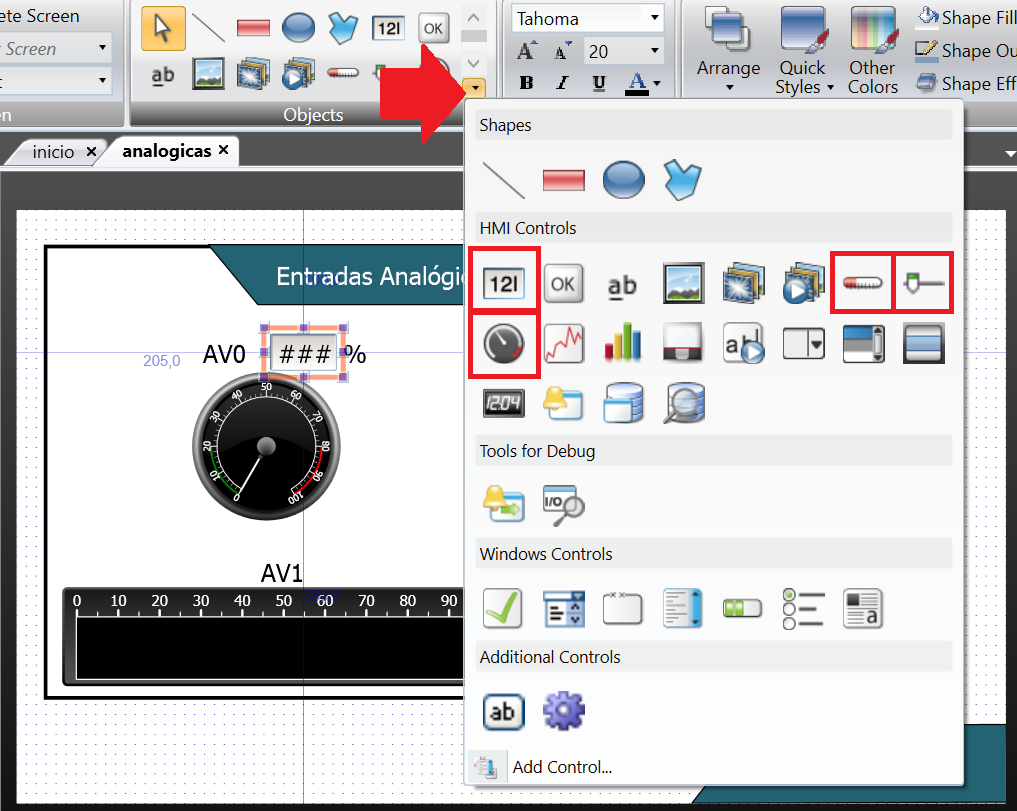
\includegraphics[width=14cm]
		{figuras/ix-analogicos_objects-n}
		}}{ \Fonte{Elaborado pelo autor}    }
\end{figure}




O mostrador analógico é um dos elementos mais simples e m
ais utilizados, inclusive, 
e alguns de seus parâmetros estão destacados na 
Figura \ref{fig:analog_meter}, 
como o apontamento da TAG que servirá de referência e
o formato do dado exibido. 
No segundo destaque o fato de ser um elemento somente de leitura,
impedindo a edição do valor exibido. 
O último destaque para o tamanho da fonte. 
Outras propriedades podem ser alteradas dependendo da necessidade funcional ou estética. 
Explore!


\begin{figure}[ht!]
	\centering
	\Caption{\label{fig:analog_meter} Mostrador analógico }
	\UECEfig{}{\fbox{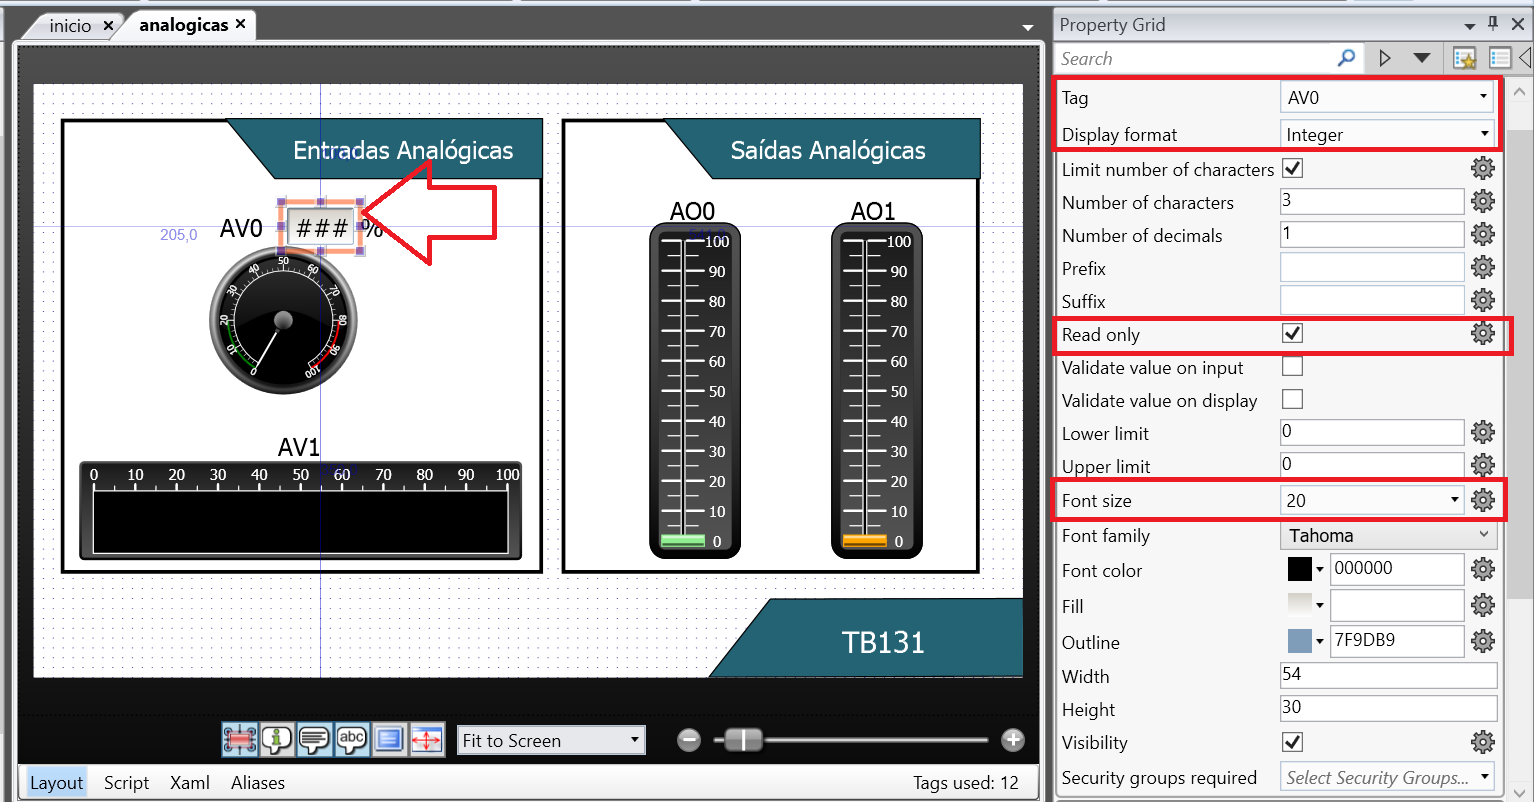
\includegraphics[width=14cm]
		{figuras/ix-analogicos_analogmeter-n}
		}}{ \Fonte{Elaborado pelo autor}    }
\end{figure}





O mostrador circular é 
o mostrador símbolo de variáveis analógicas
(mesmo que transmitidas por uma canal digital). 
A Figura \ref{fig:analog_circularmeter} 
destaca algus parâmetros dentre os muitos possíveis. 
No destaque superior é apontada a TAG de referência e 
os valores extremos de exibição. 
O destaque seguinte, 
o tipo de mostrador e o tamanho da fonte. 
O destaque inferior mostra as dimensões do objeto. 




\begin{figure}[ht!]
	\centering
	\Caption{\label{fig:analog_circularmeter} Mostrador circular }
	\UECEfig{}{\fbox{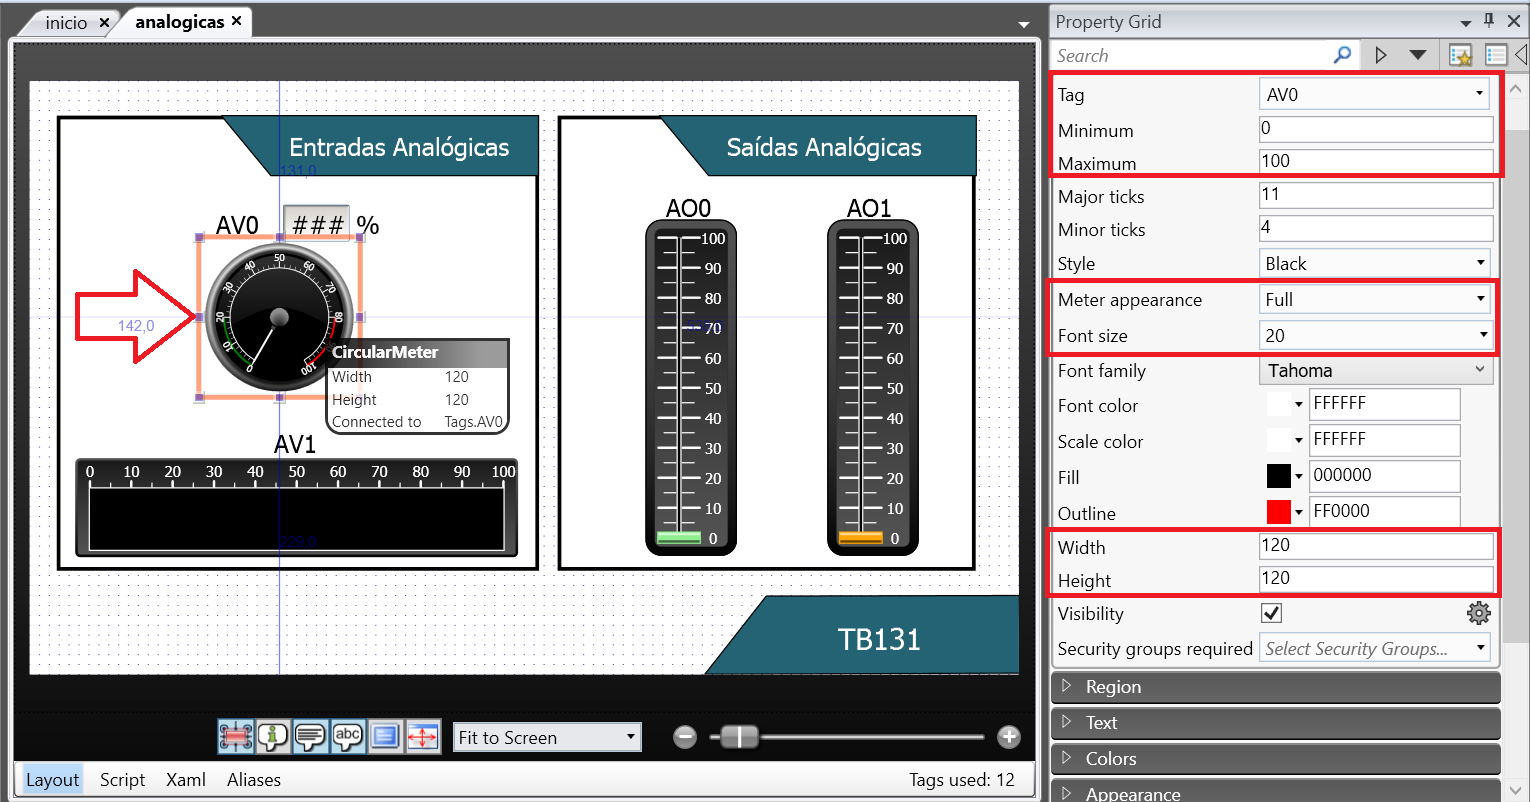
\includegraphics[width=14cm]
		{figuras/ix-analogicos_circularmeter-n}
		}}{ \Fonte{Elaborado pelo autor}    }
\end{figure}




O mostrador linear, 
possui parâmetros semelhantes ao circular,
\textbf{indicador 2},
como o apontamento da TAG de referência e os extremos de exibição,
valor máximo e valor mínimo. 


\begin{figure}[ht!]
	\centering
	\Caption{\label{fig:analog_linearmeter} Mostrador Linear }
	\UECEfig{}{\fbox{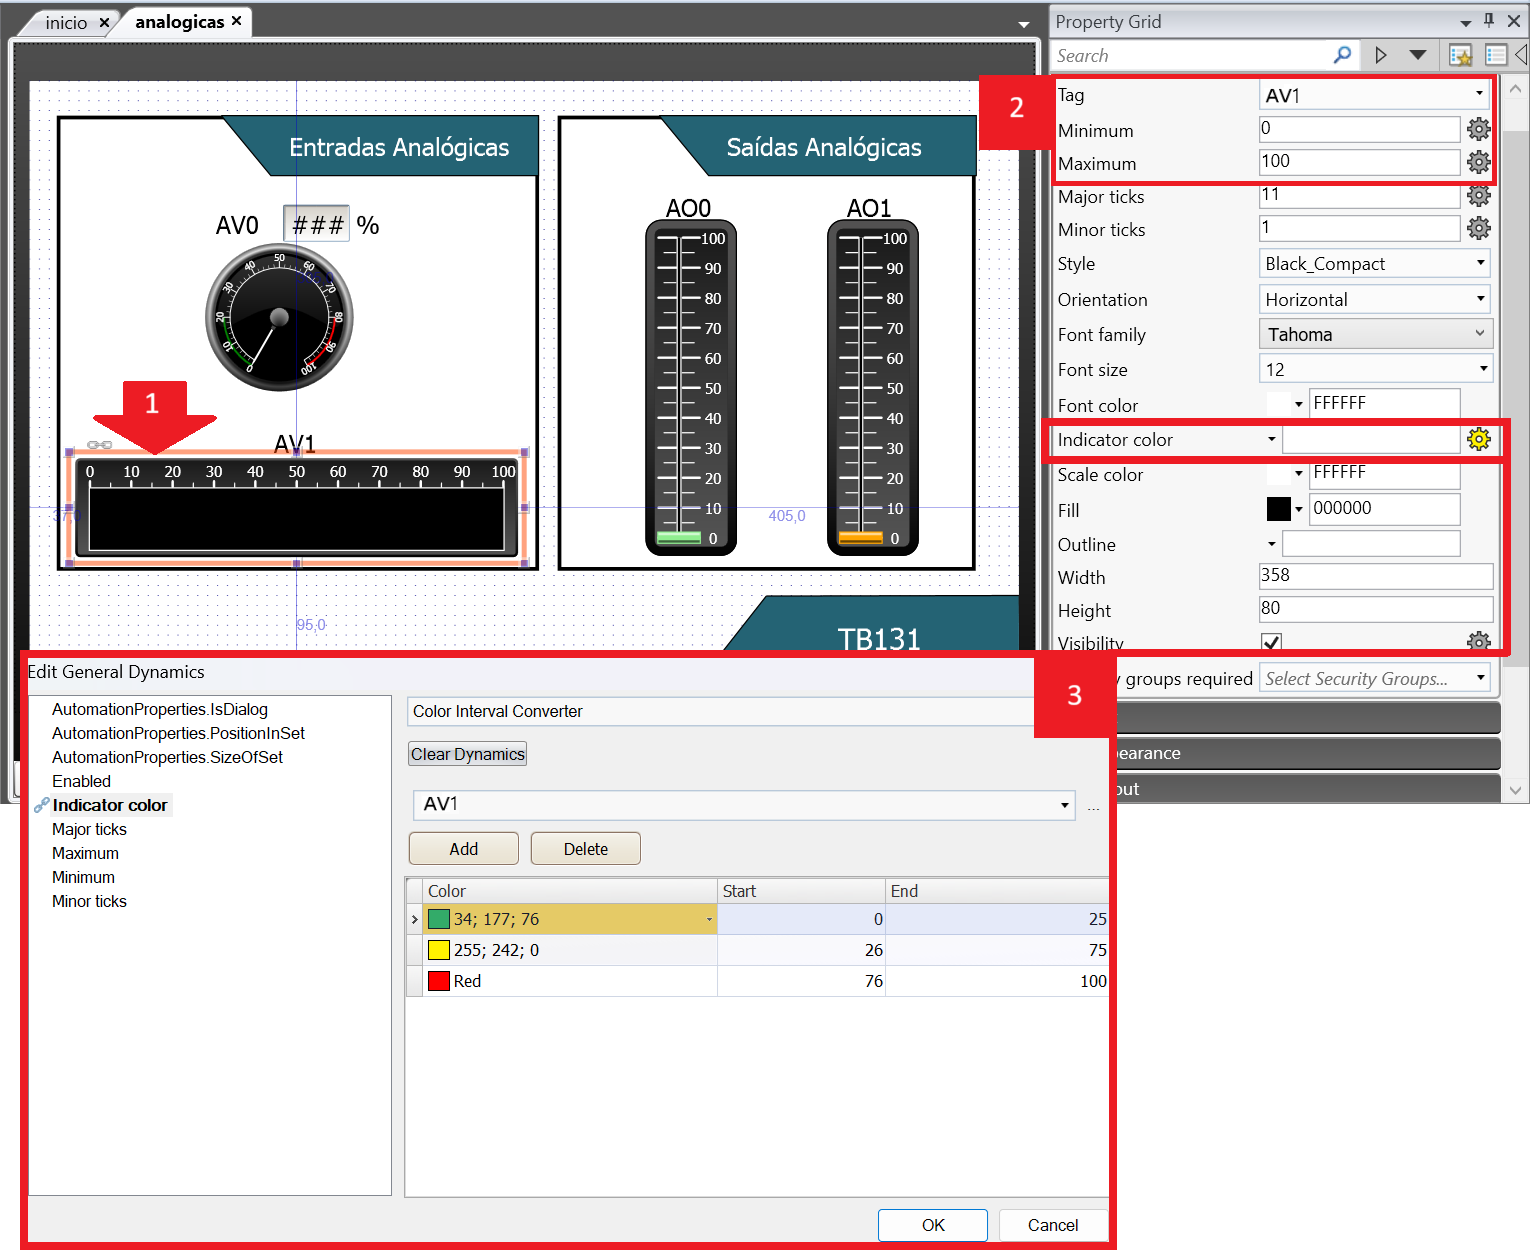
\includegraphics[width=14cm]
		{figuras/ix-analogicos_linearmeter-n}
		}}{ \Fonte{Elaborado pelo autor}    }
\end{figure}

Porém, neste caso é possível mudar a cor da barra de progresso 
a depender do valor da variável analógica de referência. 
Acessando as configurações do parâmetro 
\textbf{\textit{Indicator color}},
\textbf{indicador 3}, 
deve-se novamente indicar a TAG de referência e 
adicionar intervalos com as respectivas cores. 
O exemplo mostra a utilização de três intervalos com três respectivas cores.



Como elemento de atuação nas variáveis analógicas, 
é utilizado a objeto denominado \textbf{slider}, 
cujas propriedades são destacadas na 
Figura \ref{fig:analog_slider}. 
Assim como os demais elementos, 
deve-se apontar a TAG que servirá de referência para 
a manipulação dos dados,
\textbf{indicador 2}, 
bem como seus valores extremos.

Podem ser alterados diversos parâmetros, 
novamente, a depender da necessidade técnica ou visual, 
como a cor do elemento cursor, 
\textbf{indicador 3}. 




\begin{figure}[ht!]
	\centering
	\Caption{\label{fig:analog_slider} Chave deslizante }
	\UECEfig{}{\fbox{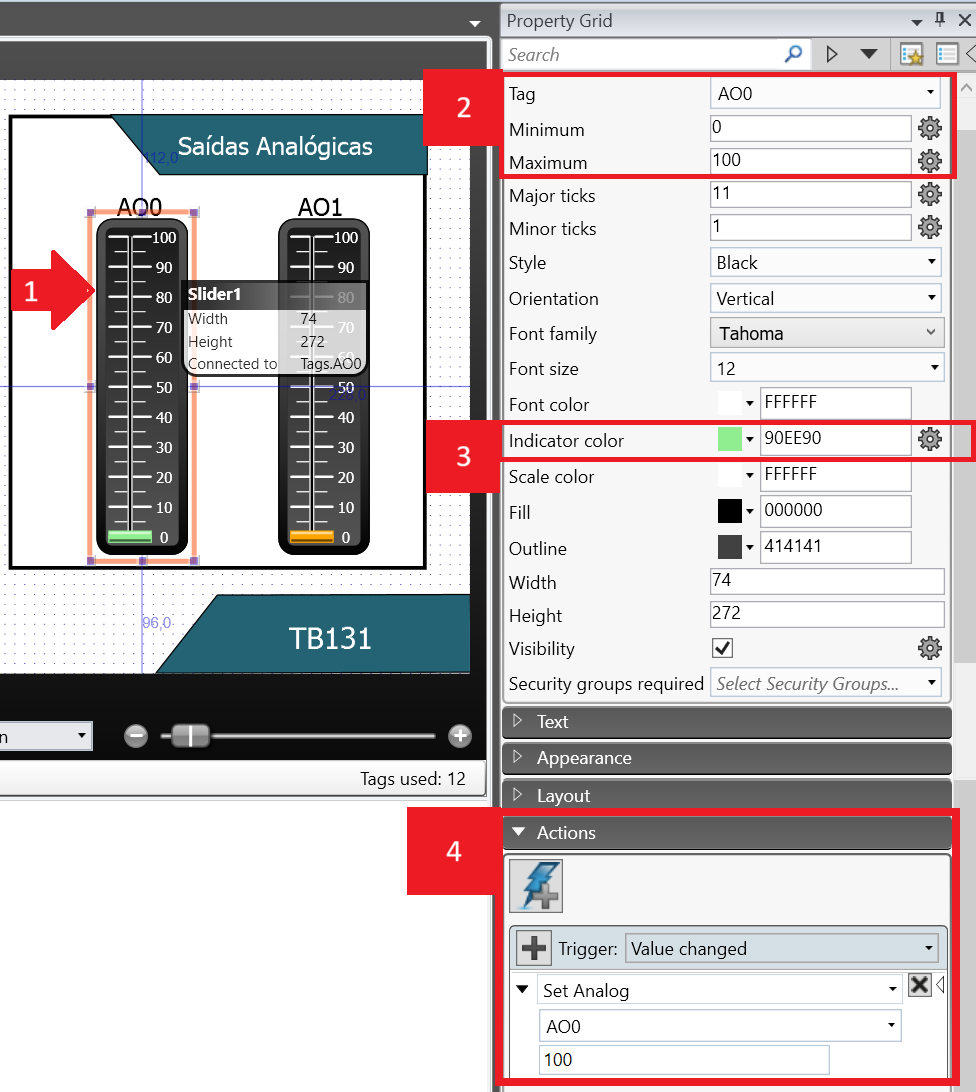
\includegraphics[width=14cm]
		{figuras/ix-analogicos_slider-n}
		}}{ \Fonte{Elaborado pelo autor}    }
\end{figure}




O parâmetro mais importante no caso de um elemento de atuação, 
é a sua configuração de ação,
\textbf{indicador 4},
em que para uma mudança de valor no seu cursor, 
ocorre a ação, 
\textbf{\textit{Set Analog}}, 
na TAG apontada e com o fundo de escala definido abaixo, 
que neste exemplo a TAG é a \textbf{AO0} 
e o fundo de escala é \textbf{100}. 


Desta forma, 
são realizadas as configurações básicas dos elementos gráficos, 
ou objetos, contidos na tela e que fazem 
a interface dos dados mediante a comunicação com o controlador.





\section{Tranferindo o projeto para o Terminal Gráfico/IHM}


Ao finalizar o desenvolimento de uma etapa do projeto, 
não somente ao final dele, 
recomenda-se que seja realizada a construção do projeto 
(\textbf{\textit{build}}), 
que consiste basicamente da compilação do que foi configurado até então, 
produzindo um arquivo executável a ser transferido ao equipamento. 

Este processo permite 
a detecção de erros de construção no projeto, 
de modo que sejam detectados o quanto antes e corrigidos.

Para este processo, 
acesse a opção \textbf{\textit{project}}, 
como na Figura \ref{fig:project_build} e 
clique em \textbf{\textit{build}},
\textbf{indicador 1}.



\begin{figure}[ht!]
	\centering
	\Caption{\label{fig:project_build} Compilação e download do projeto }
	\UECEfig{}{\fbox{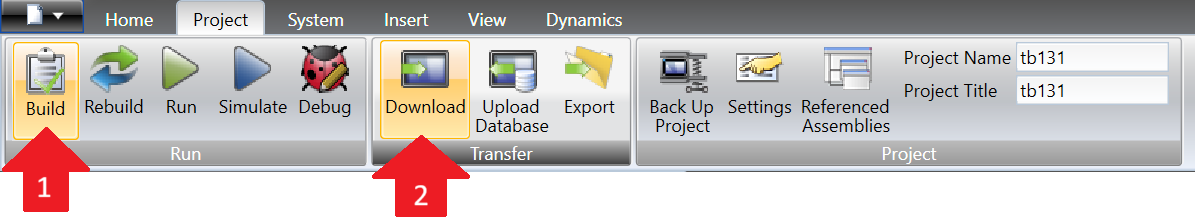
\includegraphics[width=14cm]
		{figuras/ix-project_download-n}
		}}{ \Fonte{Elaborado pelo autor}    }
\end{figure}



Na janela principal aparece o log do processo e 
ao final deve apresentar a quantidade de zero erros. 


Com isso, 
o projeto está pronto para ser transferido ao equipamento, 
clicando em \textbf{\textit{Download}}. 


Para o processo de transferência 
é necessario escolher um dispositivo alvo, 
podendo este estar conectado na mesma rede 
ou na mesma faixa de endereçamento IP. 


A Figura \ref{fig:project_download} 
ilustra um dispositivo conectado 
de forma ponto a ponto com o computador,
\textbf{indicador 1}. 
Bastando apenas clicar em \textbf{\textit{Download}} 
para inicar a transmissão. 



\begin{figure}[ht!]
	\centering
	\Caption{\label{fig:project_download} Transferência de projeto para o terminal gráfico/IHM }
	\UECEfig{}{\fbox{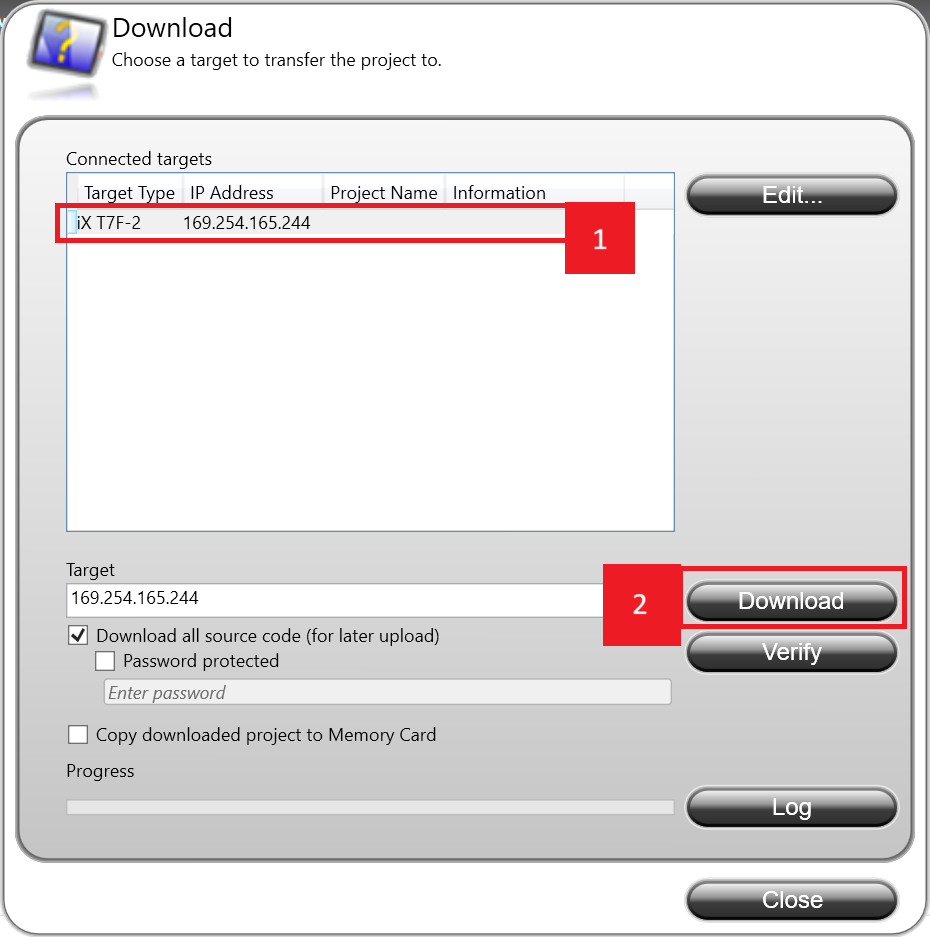
\includegraphics[width=10cm]
		{figuras/ix-project_download_ip-n}
		}}{ \Fonte{Elaborado pelo autor}    }
\end{figure}



Ao iniciar a transferência, 
o dispositivo entra em modo recepção, 
exibindo uma barra de progresso e 
mensagens de inicialização ao final do processo. 
Pode-se então fechar a janela clicando no botão 
\textbf{\textit{Close}}.

Projeto transferido ao Terminal Gráfico/IHM. 

O processo de compilação deve ser executado sempre que houver algum incremento ou ajuste no projeto, verificando assim, se não foi inserido algum erro ou falha no projeto.


